\begin{figure}[t]
\centering
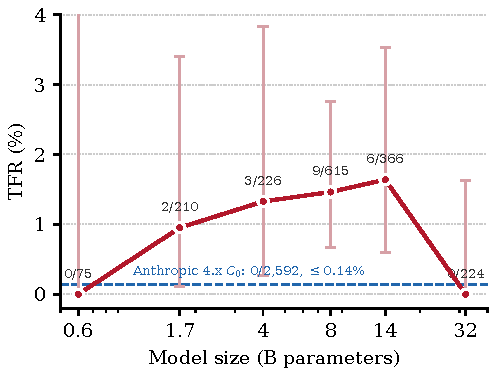
\includegraphics[width=0.98\linewidth]{figures/fig1_scaling_curve}
\caption{Qwen3-family tool-fabrication rate (TFR) under the opaque
baseline $\mathrm{C}_0$, four-distractor probe with the target tool
removed, $0.6$B--$32$B (per-call pooled; the same data as
Table~\ref{tab:qwen3-scale}). Points are pooled per-size TFR; error bars
are Clopper--Pearson $95\%$ intervals. The dashed line marks the pooled
Anthropic~4.x $\mathrm{C}_0$ upper bound ($0/2{,}592$, $\leq\!0.14\%$;
Section~\ref{sec:results:probe}), shown for reference. The shape is
non-monotone---near-zero at $0.6$B, a $\sim\!1$--$2\%$ band at $1.7$--$14$B,
and $0\%$ at $32$B---but with only six sizes and wide intervals (e.g.\ the
$32$B bound overlaps the $14$B estimate) we read it descriptively: a
single-family, single-quantization shape, \emph{not} a fitted scaling law
and \emph{not} evidence of an emergent capability. Quantization is held at
nominal $4$-bit across sizes but not at fixed reconstruction error per
checkpoint; we therefore do not attribute the shape to capability alone
(see Section~\ref{sec:limitations} and the bf16 control noted there).}
\label{fig:scaling}
\end{figure}
